\documentclass{oci}
\usepackage[utf8]{inputenc}
\usepackage{lipsum}
\usepackage{tikz}
\usetikzlibrary{shapes}

\title{Ociman y su pogo stick}

\begin{document}
\begin{problemDescription}
Ociman está a cargo del centro de operaciones de la OCI, donde se coordina la
final de la competencia y se revisan los problemas.
Para llegar a su destino sin ser visto, Ociman ha decidido usar un pogo stick,
saltando de edificio en edificio.

Vista desde arriba, la ciudad puede describirse como una grilla de $N\times N$
edificios.
Las filas y columnas son numeradas de norte a sur y de oeste a este con números
entre 1 y $N$.
Muchos de los edificios tienen techos irregulares y por lo tanto Ociman no
puede saltar sobre ellos.
Adicionalmente, Ociman tiene un límite de distancia para sus saltos y cada vez
que salta solo puede moverse a lo más $d$ edificios tanto horizontal como
verticalmente.

La siguiente imagen muestra un ejemplo para $N=6$ y $d=2$.
Los edificios sobre los cual Ociman \textbf{no} puede saltar están marcados con
una cruz.
Ociman está representado con un círculo y se encuentra en la coordenada $(3, 5)$.
El cuadrado en gris representa el área que Ociman puede alcanzar en un salto
estando en esa posición.
Dentro de ese área Ociman puede saltar a cualquier edificio que no está marcado
con una cruz.

\begin{center}
  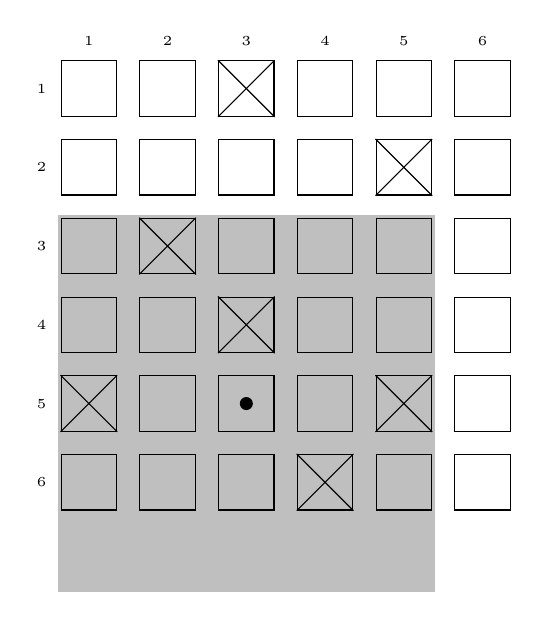
\begin{tikzpicture}[square/.style={regular polygon,regular polygon sides=4}]
    \draw [fill, lightgray] (-0.39, -1.39) rectangle +(4.78, 4.78);
    \foreach \i in {0,...,5} {
      \foreach \j in {0,...,5} {
        \node at (\i, \j) [rectangle, draw, scale=3] {};
      }
    }
    \foreach \i in {1,...,6} {
      \node at(\i-1, 5.6) {\tiny\i};
      \node at(-0.6, 6-\i) {\tiny\i};
    }
    \foreach \p in {(0,1), (2, 2), (4, 1), (4, 4), (3, 0), (1, 3), (2, 5)} {
      \node [cross out, draw, scale=2.9] at \p {};
    }
    \node [circle, fill, scale=0.5] at (2, 1) {};
  \end{tikzpicture}
\end{center}

Inicialmente Ociman comienza en el edificio en las coordenadas $(U, V)$ y tiene
que llegar al edificio en las coordenadas $(X, Y)$.
?`Cuál es el número mínimo de saltos que debe realizar para llegar a su destino? 
\end{problemDescription}

\begin{inputDescription}
La primera línea de la entrada contiene dos enteros $N$ y $d$, que corresponden
respectivamente a las dimensiones de la ciudad ($1 < N \leq 50$) y la distancia máxima
que puede saltar Ociman ($1 \le d < N$).

La segunda línea contiene dos enteros $U$ y $V$, que corresponden a las
coordenadas de la posición inicial de Ociman ($1 \le U, V \le N$).

La tercera línea contiene dos enteros $X$ e $Y$, que corresponden a las
coordenadas del edificio de la OCI ($1 \le X, Y \le N$).

Cada una de las siguientes $N$ líneas contiene $N$ enteros, describiendo una
matriz que representa la ciudad.
El $i$-ésimo entero en la línea $j$-ésima contendrá un 1 si Ociman puede saltar
sobre el edificio en las coordenadas $(i, j)$ o 0 en caso contrario.
Se garantiza que tanto la coordenada $(U, V)$ como la coordenada $(X, Y)$
contendrán edificios sobre los cuales Ociman puede saltar.
\end{inputDescription}

\begin{outputDescription}
La entrada debe consistir en un entero correspondiente al mínimo número de saltos
que Ociman debe realizar para llegar al edificio de la OCI.
Se garantiza que siempre existirá un camino válido.
\end{outputDescription}

\begin{scoreDescription}
  % TBD distribución de puntajes
  \score{25} Se probarán varios casos donde Ociman puede saltar sobre todos los
  edificios, es decir, la matriz que describe la ciudad tiene solo unos.
  \score{75} Se probarán varios casos sin restricciones adicionales.
\end{scoreDescription}

\begin{sampleDescription}
\sampleIO{sample-2}
Este caso corresponde al ejemplo de la figura.
Ociman puede saltar a la posición (5, 3) y luego a la posición (5, 1), donde se encuentra el edificio de la OCI.

\sampleIO{sample-1}
Ociman parte en la posición (3, 4).
Desde allí puede realizar la secuencia de saltos (3, 4) $\rightarrow$ (4, 3) $\rightarrow$ (4, 2) $\rightarrow$ (4, 1).

\end{sampleDescription}

\end{document}
